\chapter{Experimental apparatus}

The working principle of this experiment is based on one of Rasetti's 1941 experiments where he first measured resting muon's lifetime through a coincidence circuit.

\section{Experimental principle}

\begin{figure}[htbp]
\centering
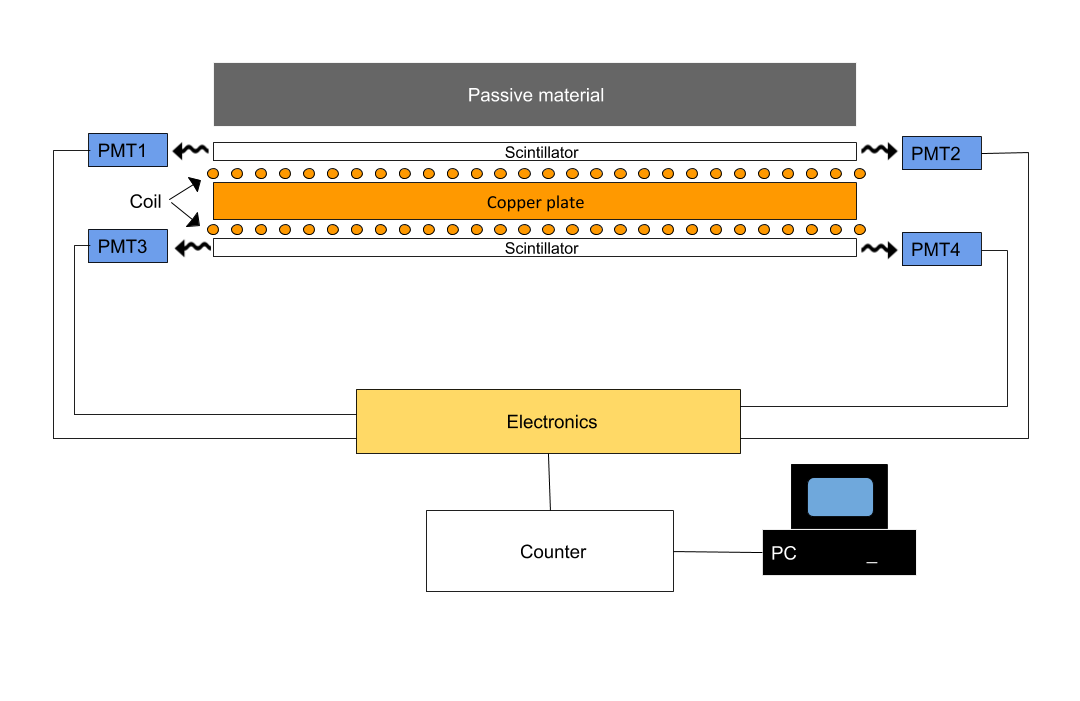
\includegraphics[width=\linewidth]{./fig/principle.png}
\caption{Illustration of the experimental apparatus.}
\label{fig:principle}
\end{figure}

Figure \ref{fig:principle} describes the experiment's principle. The Copper target stops muons and is placed inside a magnetic field. The muon's lifetime is measured by looking at the time between a muon's stopping and the emission of a positron. The preferred direction direction and the Larmor frequency must also be registered in order to determine the magnetic moment. Particles are detected through scintillator plates. Scintillators are materials which, when ionized, will rearrange their electronic structures and emit photons at set energies. Those scintillators are connected to wave guides and further to photomultipliers (here Photo-Multiplier-Tubes or PMTs), which then convert the light signal into an electronic one. The times are then saved on a PC. In other to provide further shielding to the experiment, a \SI{5}{\centi\meter} layer of dense and passive material (here lead) is added on top of the experiment.

A muon stop is experimentally defined as an electronic signal signal from the coincidence circuit of \textit{PMT 1} and \textit{PMT 2} but none from that of \textit{PMT 3} and \textit{PMT 4}. Indeed an unstopped muon would traverse both scintillator layers and would thus register a signal in both coincidence circuits. In the logic language, a stopped muon would thus be written as:

\begin{equation}
(\text{\textit{PMT 1}} \;\text{\textbf{AND}} \; \text{\textit{PMT 2}}) \; \text{\textbf{AND}} \; (\overline{\text{\textit{PMT 1}}} \; \text{\textbf{AND}} \; \overline{\text{\textit{PMT 2}}}).
\end{equation}

Two PMTs and a coincidence circuit are used so as to rule out random events, muons generate strong photon bursts that can be seen by both PMTs. A muon decay is defined in the same way as a muon stop meaning that when a particle is sent downwards, it isn't registered, leading to a loss in statistics.

Nevertheless, this logic circuit is used because there would otherwise be no spatial resolution and thus no way to determine the muon spin which is needed for the magnetic moment determination. Since muon stops and decays are registered as the same signal, the two events need to be seperated through their sequence:

\begin{itemize}
\item A muon decay is a stochastic process which thus is distributed according to an exponential probability distribution. For an average lifetime of $\tau=\SI{2.2}{\micro\second}$ we get a half-life $\lambda=\frac{\tau}{\ln(2)}\simeq \SI{1.5}{\micro\second}$, therefore $99\%$ of muons decay after $\SI{10}{\micro\second}$.
\item Due to the low vertical radiation intensity, the average distance between two muons is $\sim\SI{10}{\second}$ which is about 10 times the $\SI{12.5}{\micro\second}$ readout length.
\end{itemize}

Thus, an event is identified as a muon-stop if and only if a second event takes place in the next \SI{12.5}{\micro\second} which then defines a decay. All other events are discarded.


\section{Target and B-field}

Muon are captured in a \SI{1}{\meter} long, \SI{50}{\centi\meter} wide and \SI{2.5}{\centi\meter} thick copper plate. Copper as a material has the following advantages justifying its use:

\begin{itemize}
\item It is slightly diamagnetic ($\chi_{\text{m}}=-7.4 \cdot 10^{-6}$) and thus has little influence over the magnetic field.
\item Its thickness allows it to effectively stop muons.
\item The muons are not depolarized by the formation of muonium.
\end{itemize}

The coil used in this experiment is \SI{1}{\meter} and composed of 456 loops. The calibration curve in Figure \ref{fig:magcal} shows the need for $\SI{10}{\ampere}$ for $\SI{48}{\gauss}$ (calibration $B[Gauss]=\SI{4.72}{\text{I}}$) and thus, a $\SI{4.1}{\mega\hertz}$ Larmor Frequency $\omega_{\text{L}}$. This corresponds to a period $T=\frac{2\pi}{\omega}$ so $\sin \SI{1.5}{\micro\second}$, which, with a time resolution of $\SI{0.05}{\micro\second}$ and a window of $\SI{12.5}{\micro\second}$, such as in this experiment, theoretically 7-8 periods should be observed.

\begin{figure}[htbp]
\centering
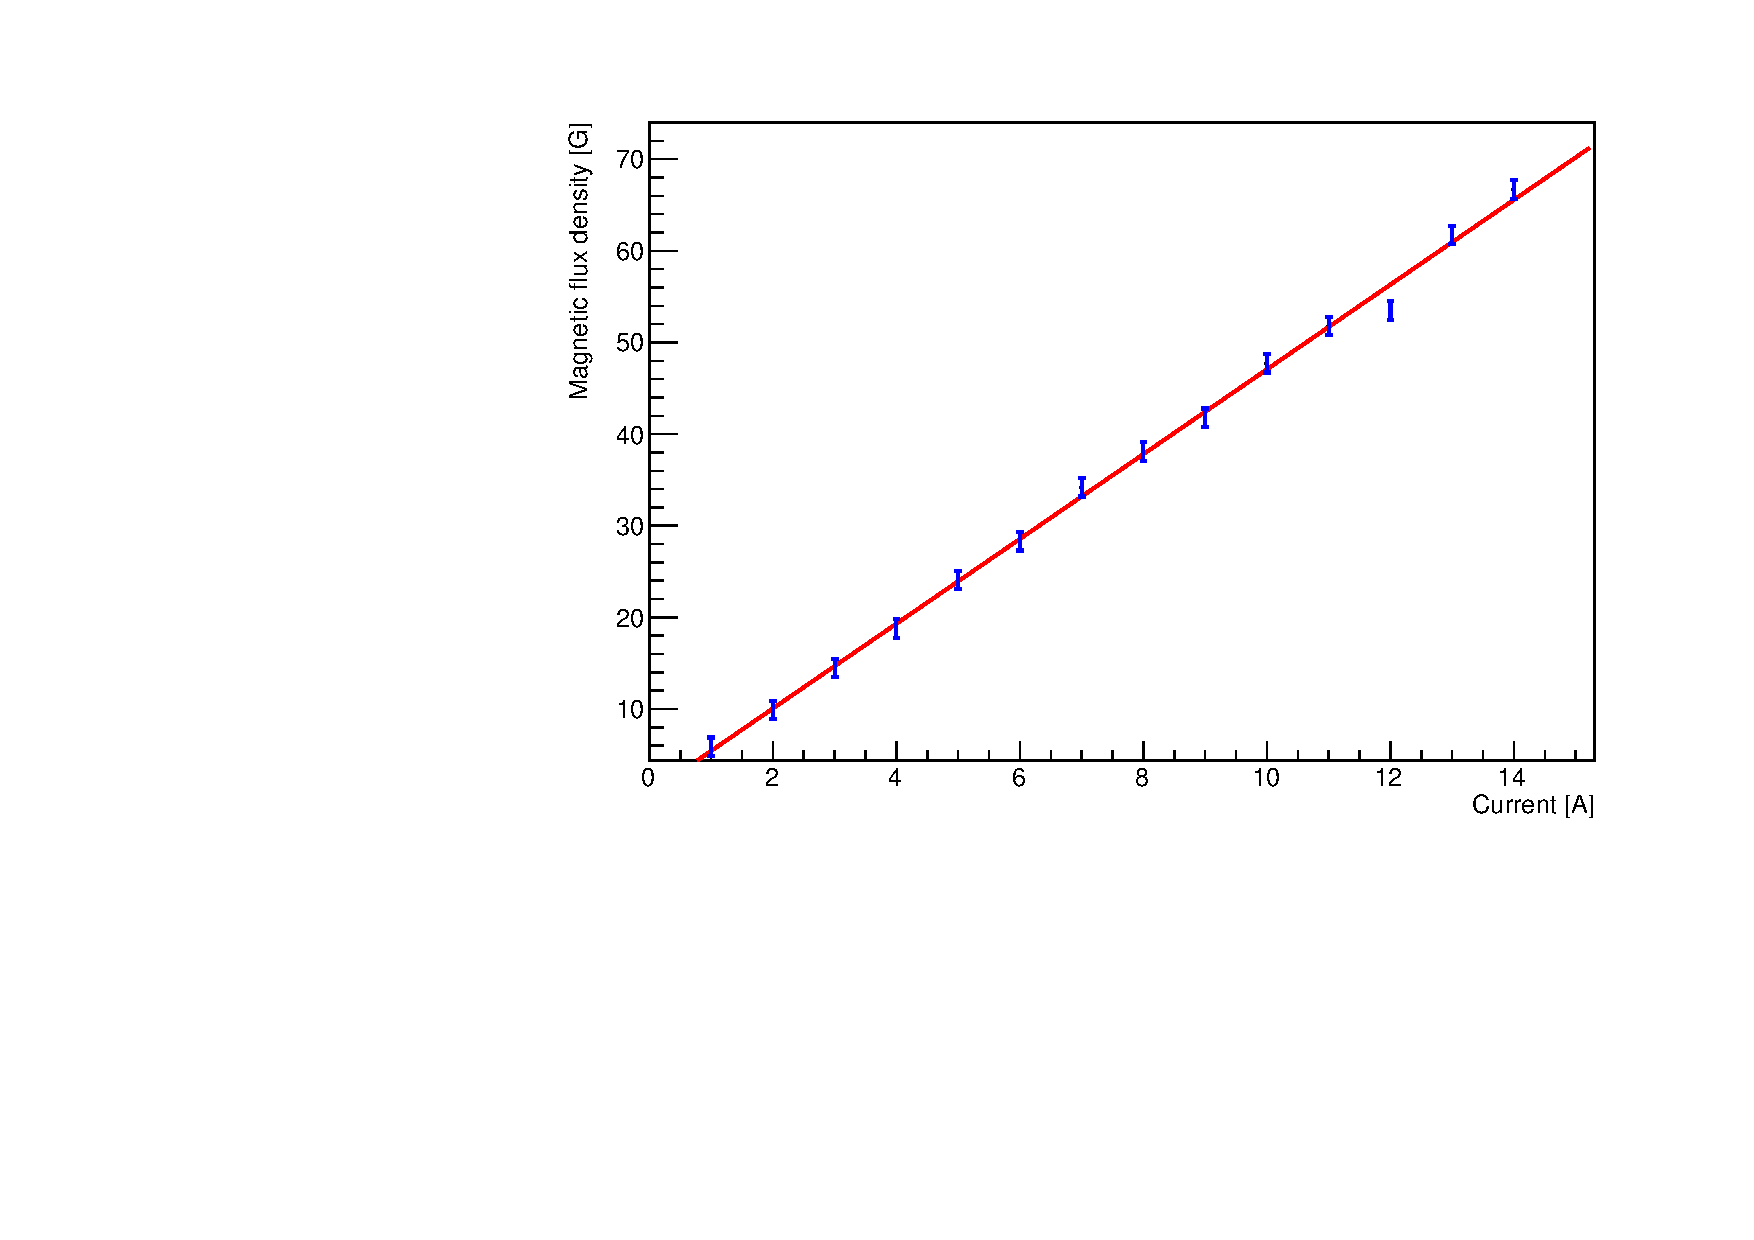
\includegraphics[width=0.7\linewidth]{./fig/magcal.pdf}
\caption{Calibration curve of the magnetic field as measured with a fluxgate compass.}
\label{fig:magcal}
\end{figure}


The magnetic field must however be homogenous enough that two muons stopped at different locations don't have too big of a phase difference. If the relative phase difference should be $\Delta\omega T \leq 0.3$, with $T$ being the measurement period (i.e. \SI{12.5}{\micro\second}). In this case, equation \ref{eq:larm} implies that the homogeneity of the B-field at \SI{48}{\gauss} must satisfy $\frac{\Delta B}{B}\leq 0.008$. If one uses the law of Biot-Savart to compute the magnetic field, they would find $\frac{\Delta B}{B}=0.013$. An additional \SI{10}{\centi\meter} long correction coil at each end of the main coil improves the value to 0.008. Calculations with different current values show that this value represents an absolute minimum for this arrangement and is achieved precisely when the correction coil current is half of that of the main coil. The secondary coils are thus connected in parralel to each other and in series with the main one as shown in Figure \ref{fig:coil}.

\begin{figure}
\centering
   \begin{subfigure}[t]{0.49\linewidth}
  \centering
   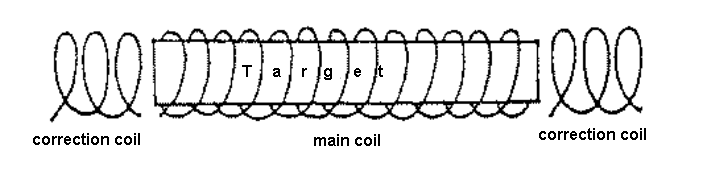
\includegraphics[width=\linewidth]{./fig/coil1.png}
  \caption{}
\label{sfig:coil1}
  \end{subfigure}
   \begin{subfigure}[t]{0.49\linewidth}
  \centering
   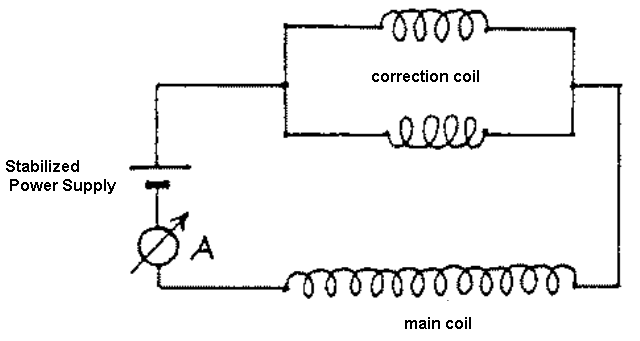
\includegraphics[width=\linewidth]{./fig/coil2.png}
  \caption{}
\label{sfig:coil2}
  \end{subfigure}
\caption{(a) Magnetic coil structure. (b) Magnetic coil circuit.}
\label{fig:coil}
\end{figure}

\begin{figure}
\centering
 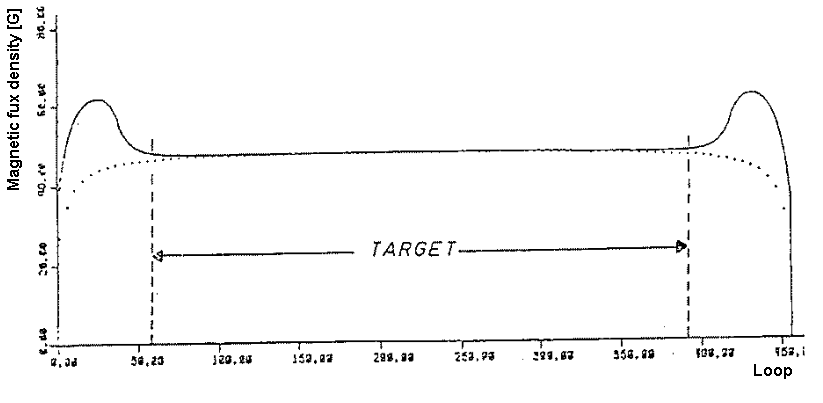
\includegraphics[width=\linewidth]{./fig/coillength.png}
\caption{Magnetic field as calculated along the coil at \SI{10}{\ampere}.}
\label{fig:fieldstr}
\end{figure}

\begin{figure}
\centering
 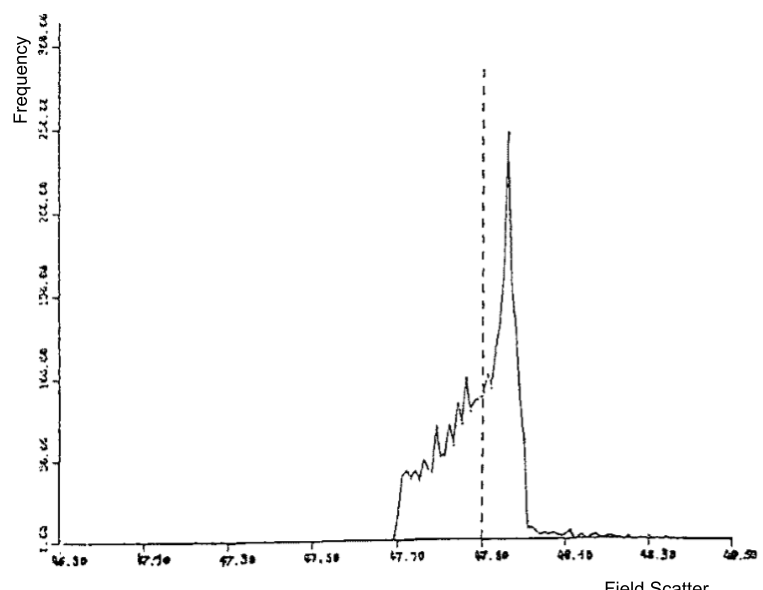
\includegraphics[width=\linewidth]{./fig/fieldscat.png}
\caption{Scatter of the B-field as calculated along the coil axis for a \SI{10}{\ampere} current. The dotted line represents the average scatter.}
\label{fig:fieldscat}
\end{figure}

The homogenity of the magnetic field is shown in Figures \ref{fig:fieldstr} \ref{fig:fieldscat}.
The temporal stability of the magnetic field's current is ensured through a stabilized power supply up to $0.5 \%$. The deterioration of $\frac{\Delta B}{B}$  by a further 0.005 such as to not observe the muon's polarization over the measurement period of \SI{12.5}{\micro\second}. In order to cool the coil, which is always powered at \SI{10}{\ampere}, a ventilator, which \textbf{always needs to be turned on when the B-field is in use}, is used.

\section{Particle detection apparatus}

The scintillators above and below the copper target are of type NE110 (organic scintillator) have a surface of $90 \times \SI{45}{\centi\meter\squared}$. As the ionizing particles pass through the scintillator, the molecular electron states are being excited, this leads to de-excitation with emission of UV light. Since the absorption length of this UV light is very short, it will be absorbed by another scintillator atom which will lead to a similar electronic process and the isotropic emission of another, shorter wavelength fluorencence photon. It is thus also called a wavelength shifter. The fluorescent decay time is of the order of $\SI{e-10}{\second}$. In order to loss of signal, the scintillator surface is polished and covered in aluminized foil, this reflects photons that would otherwise exit the scintillator. In other to deal with background from ambient light, photographic paper covered in black foil forms an outer layer of the scintillator units.

\section{The photomultiplier}

The light produced in the scintillators is guided in a plexiglas waveguide to a photomultiplier. A photomultiplier is an electronic detector used to convert light into electrons. The photomultipliers used here are Photo-Multiplier-Tubes (PMT) shown in Figure \ref{fig:PMT} a widely used technology for light detection. The photomultiplier tube is based on a thin vapour-deposited conducting layer photocathode which converts photons to electrons via the photoelectric effect, these electrons are then pass through a focusing electrode directing them towards a dynode circuit serving to amplify the electron signal via secondary emission \cite{Dekker1981}. Each dynode is held at at slightly higher ($\sim \SI{100}{\volt}$) potential than the preceding one. When an electron strikes a dynode, it will cause emission of low energy electrons which will then be accelerated towards the next dynode. The geometry of the dynode circuit is such that a cascade occurs with an exponentially increasing number of electrons being produced at each dynode. The final dynode is connected to an anode, since at this stage, a large number of electrons reach the anode, it will create a sharp rising edge which is an easy analogue signal to detect. The voltage distribution in the dynodes is done through a voltage divider circuit. The photocathode is generally held at a negative high voltage of order 1000 V, while the anode is very close to ground potential. The capacitors across the final few dynodes act as local reservoirs of charge to help maintain the voltage on the dynodes while electron avalanches propagate through the tube. It should be noted that the design shown in Figure \ref{sfig:PVD} is only an example as many different such circuits exist.

\begin{figure}
\centering
   \begin{subfigure}[t]{0.49\linewidth}
  \centering
   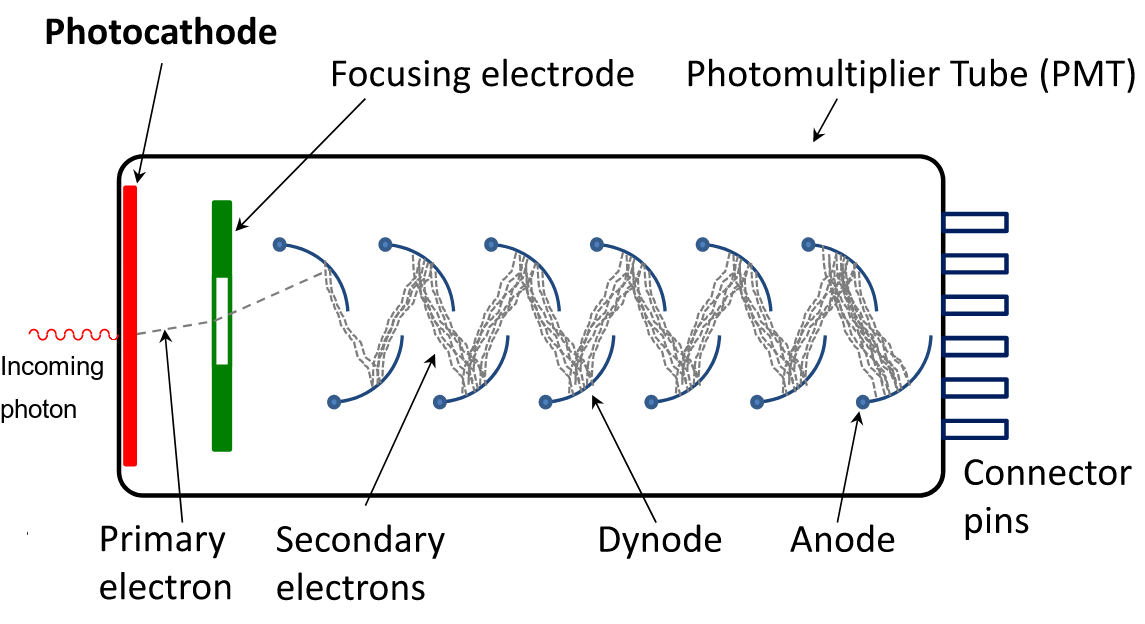
\includegraphics[width=\linewidth]{./fig/PMT.png}
  \caption{}
\label{sfig:PMT}
  \end{subfigure}
   \begin{subfigure}[t]{0.49\linewidth}
  \centering
   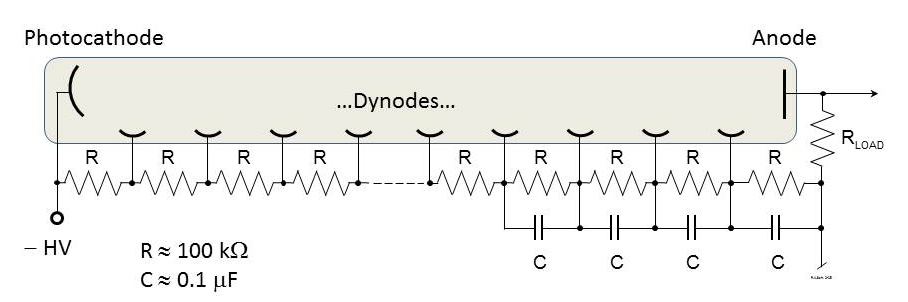
\includegraphics[width=\linewidth]{./fig/PMT_Voltage_Divider.jpg}
  \caption{}
\label{sfig:PVD}
  \end{subfigure}
\caption{(a) PMT schematic illustration. (b) PMT example voltage divider circuit \cite{wiki}.}
\label{fig:PMT}
\end{figure}


\section{Electronics}

The PMTs emit short, fast, subsequent electronic impulses, the electronics are used to discriminate muon-stop signals. This happens with a coincidence circuit. A coincidence can be seen as a an "electronic binary operator" (through an \textbf{AND} gate), it thus takes two signals as inputs which in the case of the Nuclear Instruments Module (NIM), take gate signals with binary values of \SI{700}{\milli\volt} (logical 1/\textbf{TRUE}) or \SI{0}{\volt} (logical 0/\textbf{FALSE}). It provides a fixed output based on the mode of operation either a gate signal or a logical 0. The coincidence can be operated as \textbf{AND} ($\odot$), \textbf{OR} ($\oplus$), \textbf{NAND} (=$\overline{\text{\textbf{AND}}}$) or \textbf{NOR} ($=\overline{\text{\textbf{OR}}}$). The output signal depends on the input algebra logic which can be found in Table \ref{tab:log}.

The conditions for a muon stop or decay from Figure \ref{fig:principle} can be written:

\begin{equation}
\big(\text{PMT}1 \odot \text{PMT}2\big) \odot \big(\overline{\text{PMT}1} \oplus \overline{\text{PMT}2}\big).
\end{equation}

The first block represents a logical \textbf{AND} while the second one represents a logical \textbf{NOR} (see Table \ref{tab:log}). The entire logical circuit, including the \textbf{AND} is realized in the electronic circuit shown in Figure \ref{fig:elek} in coincidences 1,2 and 3. The logical units used to make coincidences require sharp rectangular gate (digital) pulses which is why the analog PMT signal is connected to discriminators after amplification. Similarly to the coincidences, the discriminator output length can be varied. Discriminators also include the possibility to separate interference pulses (noise) from signal: they will only deliver a gate signal if the signal input exceeds a certain threshold which can be set. The rest of the circuit after coincidence 3 is used to set a counter to measure the decay time, from the start of a muon-stop (Reset) and stop at the subsequent event (interrupt) if this occurs within the fixed \SI{12.5}{\micro\second}. The counter reset and the \SI{12.5}{\micro\second} wide time window are implemented via the monoflop. A monoflop has one input ($s$) for start (as the reset is only used when operating as a flip-flop) and three outputs:

\begin{itemize}
\item $o$ (out) produces a gate output of variable length caused by an input and a \SI{0}{\volt} output otherwise.
\item $\overline{o}$ ($\overline{\text{out}}$) which produces an opposite signal to o.
\item $e$ (end) sends a short gate output of fixed length (per example \SI{10}{\nano\second}) when the output signal has ended.
\end{itemize}

\begin{figure}[htbp]
\centering
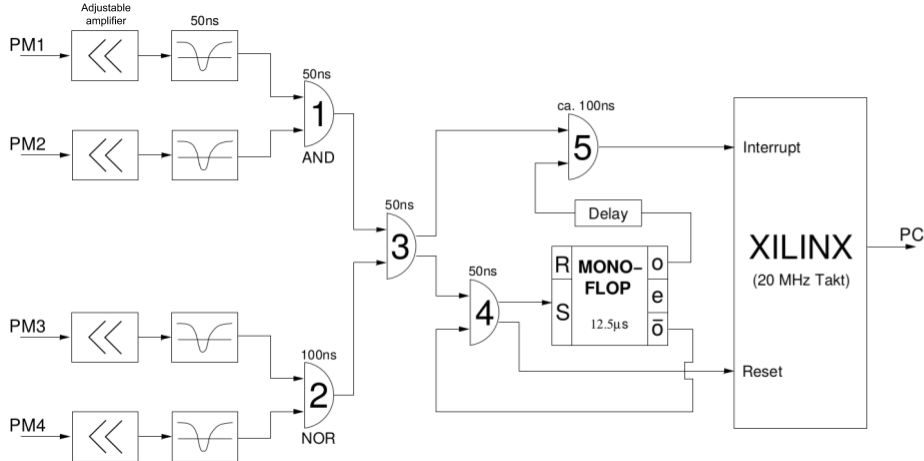
\includegraphics[width=0.7\linewidth]{./fig/electronicc.png}
\caption{Electronic circuit of the experiment.}
\label{fig:elek}
\end{figure}

\begin{table}
\begin{tabular}{|c|c|c|c|c|c|}
\hline
Input $\text{S}_1$ & Input $\text{S}_2$ & \textbf{AND} ($\odot$) output & \textbf{OR} ($\oplus$) output & \textbf{NAND} ($\overline{\text{\textbf{AND}}}$) output & \textbf{NOR} ($\overline{\text{\textbf{OR}}}$) \\ \hline
1 & 1 & 1 & 1 & 0 & 0 \\
1 & 0 & 0 & 1 & 1 & 0 \\
0 & 1 & 0 & 1 & 1 & 0 \\
0 & 0 & 0 & 0 & 1 & 1 \\ \hline
\end{tabular}
\caption{Coincidence logic table.}
\label{tab:log}
\end{table}


The monoflop open with a \SI{12.5}{\micro\second} gate for coincidence 5 and blocks coincidence 4 so that the reset switch isn't hit during the measurement period. Coincidence 5 is then ready for \SI{12.5}{\micro\second} to receive the second, supposedly delayed second signal from coincidence 3 and thus stop the counter.

The variable delay between monoflop and coincidence is achieved through an extra cable. It is crucial that signals from coincidence 3 nd the monoflop be perfectly spaced out since the start signal cannot be allowed to overlap with the gate so as to immediately trigger a reset. On the other hand, dead time between the start signal and the start of the gate (which is accepted as a stop) cannot take place either.

\section{Time measurement}

The time between the first, muon-stop, signal and the ensuing signal (muon decay) will be determined with a \textit{Time to Digital Converter} (TDC). This TDC is done with a \textit{Field Programmable Gate Array} (FPGA) from XILINX. An FPGA can be seen as an array of programmable logic blocks not unlike the coincidences described earlier. The blocks and their connections are programmed in by the user. Interactions with the outside world is done through I/O blocks. A network of programmable connections is available for connections between individual blocks.

The TDC is here programmed so as to function similarly to an 8-bit counter, which is reset through the aforementionned Reset-signal. Until the interrupt signal is received, the value of the counter is incremented by one unit for every XILINX board cycle. The clock frequency of the board is 20 MHz which corresponds to a counting unit of \SI{50}{\nano\second} and thus yields a maximum counted time difference is \SI{12.8}{\micro\second}. If the interrupt signal is received within this time, the counter's value is readout by the software on the connected PC	and converted into a time value.


\section{Data acquisition with the PC}

4-5 \si{events\per\minute} are expected. This counting rate thus requires to extend the measurement period to a week in order for enough statistics to be gathered. The DAQ program works as follows: when the XILINX obtains a valid event, its counter's value is sent to the PC and converted there into a time value. This value is then histogrammed which has 256 bins of \SI{50}{\nano\second}, corresponding to the range of all possible values that can be outputed by the TDC. The time measurements are then plotted and saved for every event (allowing for data recovery in the case of a crash or the like). The data is written into files which can be then easily be read-out. The DAQ software is in german but a measurement can be started by going into \textit{Messung}$\rightarrow$\textit{Beginnen} and ended through \textit{File}$\rightarrow$\textit{Beenden}, the measurement GUI and window can be found in Figure \ref{fig:MP}.

\begin{figure}
\centering
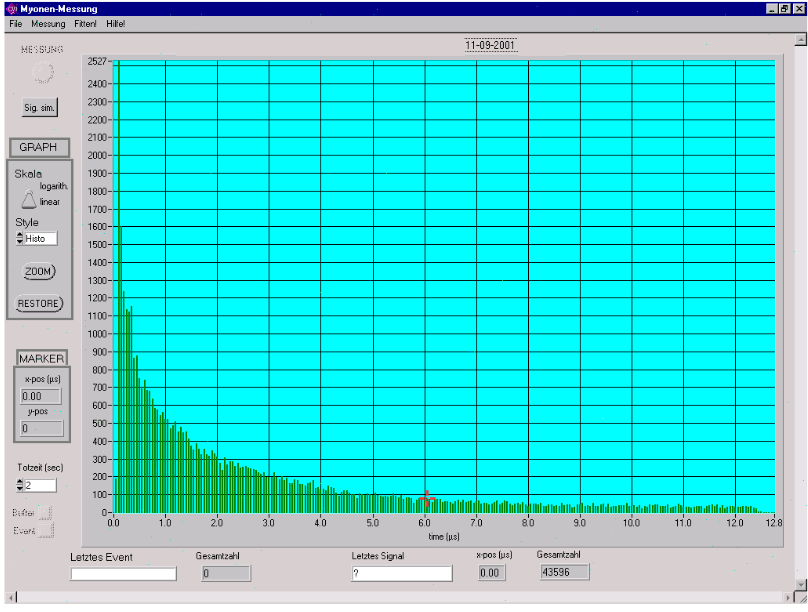
\includegraphics[width=\linewidth]{./fig/MP.png}
\caption{Measurement software window.}
\label{fig:MP}
\end{figure}
